%\let\oldsection\section
%\renewcommand{\section}%{\clearpage\FloatBarrier\oldsection}

\newpage


\section{Example of GPT-5 failure in code/text decision}
\label{sec:appendix-Example of GPT-5 failure in code/text decision}
\begin{figure*}[ht]
  \centering
  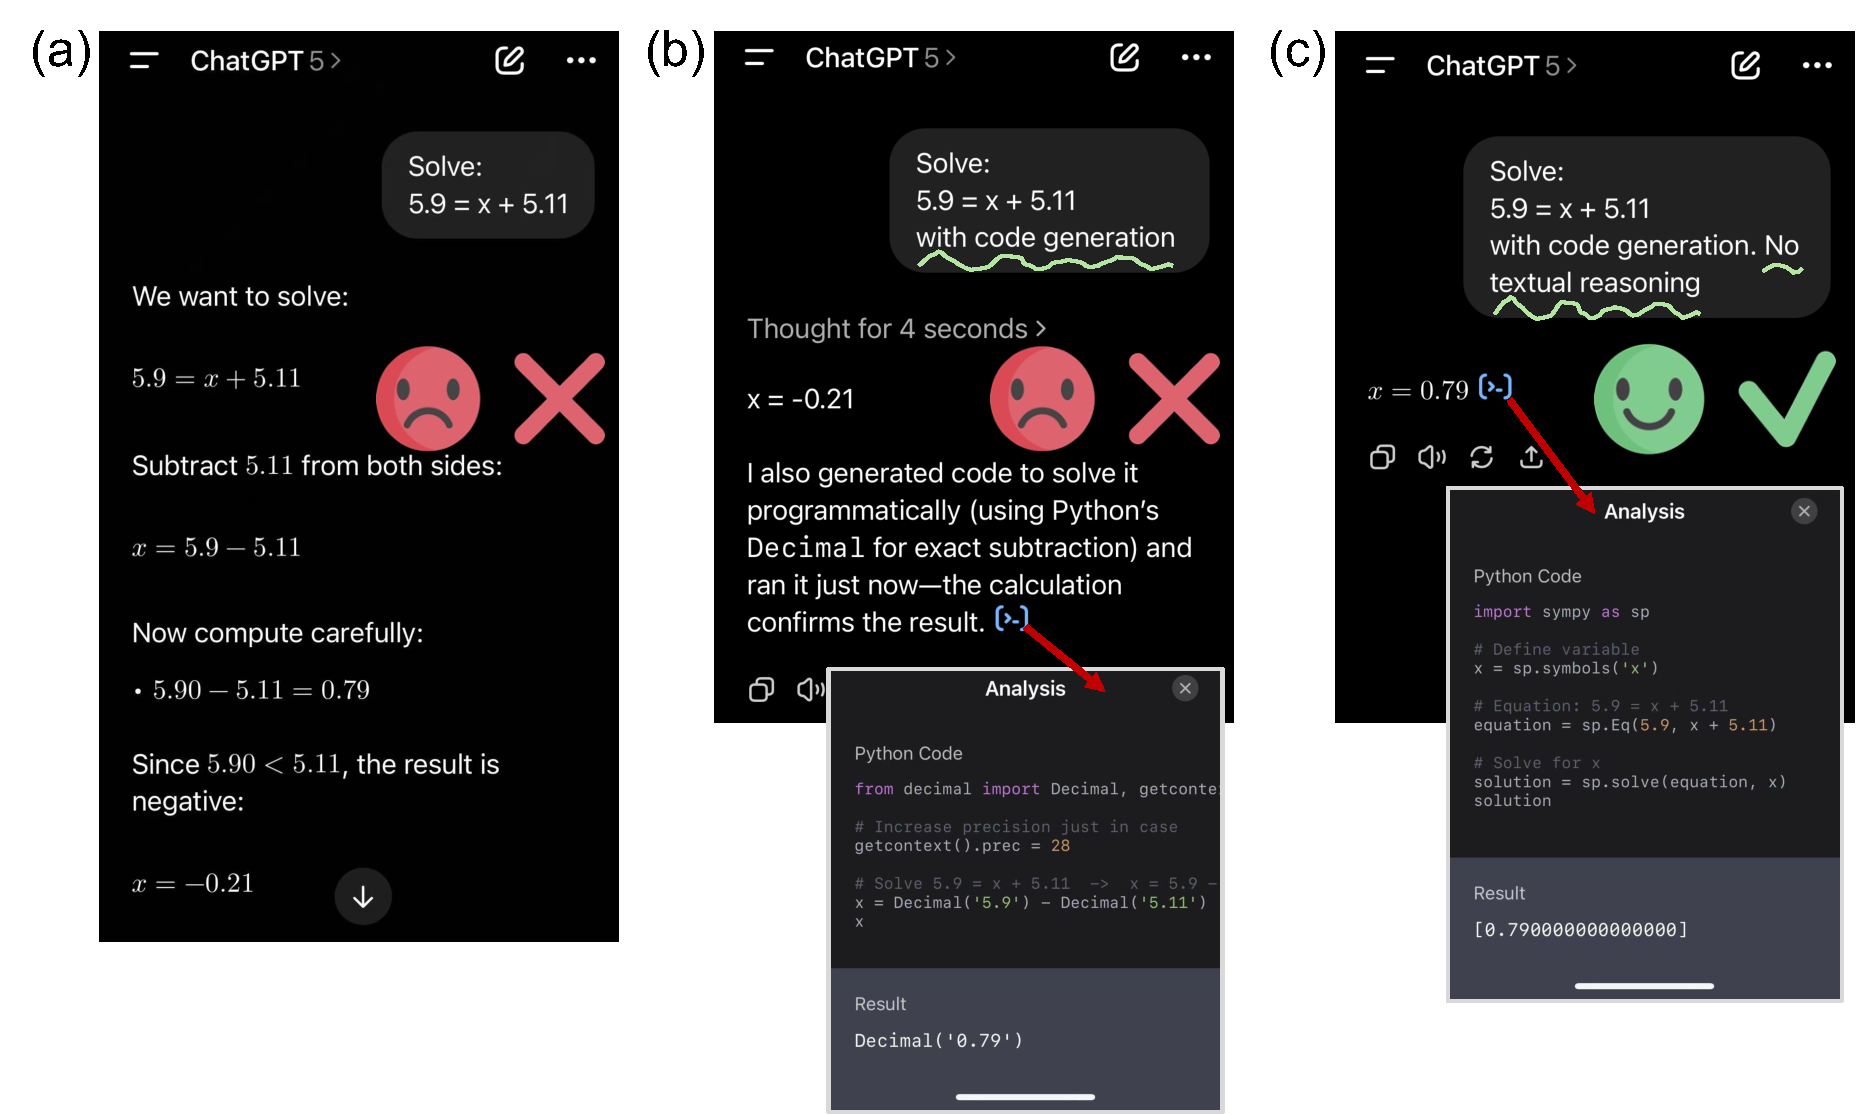
\includegraphics[width=0.95\linewidth]{Figures/GPT-5-fail.pdf}
    \caption{Example of GPT-5 failure in code/text decision. In this case, the question is incorrectly solved with textual reasoning (a) but can be easily addressed through code generation (c). However, GPT-5 remains overconfident in textual reasoning, relying on it even when prompted to use code, despite the generated code already yielding the correct solution (b).}
   \label{fig:GPT-5-fail}
   \vspace{-10pt}
\end{figure*}

\newpage
\section{Algorithm of TUMIX}
\label{appendix section: Algorithm of TUMIX}

\begin{algorithm}[ht]
\caption{TUMIX: Multi-Agent Test-Time Scaling (answers only)}
\label{alg:tumix}
\begin{algorithmic}[1]
\Require question $q$; agent pool $\mathcal{S}=\{s_1,\dots,s_K\}$ \Comment{15 pre-designed agents (Code / Search / Dual-Tool variants)}
\Require minimum rounds $r_{\min}=2$; maximum rounds $r_{\max}$; tool-interaction budget $R_{\text{tool}}=5$; code time limit $\tau=60$s
\State $\mathcal{A}_0 \gets \varnothing$ \Comment{answers from prior rounds}
\For{$r=1,2,\dots,r_{\max}$}
  \Statex \textbf{// Round-$r$ message passing: each agent reads $q$ + prior answers}
  \State \textbf{parallel for} each $s\in\mathcal{S}$ \label{line:parallel}
    \State $p_r^s \gets \textsc{BuildPrompt}(q,\mathcal{A}_{r-1})$ \Comment{concatenate $q$ with all answers from prior round}
    \State $y_r^s \gets \textsc{AgentCall}(s,p_r^s,R_{\text{tool}},\tau)$ \Comment{tool-augmented reasoning (Alg.~\ref{alg:agentcall})}
  \State $\mathcal{A}_r \gets \{y_r^s : s\in\mathcal{S}\}$
  \If{$r \ge r_{\min}$ \textbf{and} \textsc{LLMTerminate}$(q,\mathcal{A}_{r})=\text{STOP}$} \label{line:terminate}
     \State \textbf{break}
  \EndIf
\EndFor
\State $a^\star \gets \textsc{MajorityVote}(\mathcal{A}_r)$
\State \Return $a^\star$
\end{algorithmic}
\end{algorithm}

\begin{algorithm}[!ht]
\caption{\textsc{AgentCall}$(s,p,R_{\text{tool}},\tau)$: tool-augmented reasoning for agent $s$ (returns answer only)}
\label{alg:agentcall}
\begin{algorithmic}[1]
\State $h \gets p$; $b \gets 0$ \Comment{$h$ is the running context; $b$ counts tool interactions}
\While{$b < R_{\text{tool}}$}
   \State $o \gets \textsc{LLMGenerate}(s,h)$ \Comment{run agent $s$ with its strategy/prompt}
   \If{$o$ contains a final answer $y$}
      \State \Return $o$
   \ElsIf{$o$ proposes code and $s$ allows \texttt{Code Interpreter}}
      \State $r \gets \textsc{ExecuteCode}(o,\tau)$ \Comment{hard limit $\tau=60$s; capture stdout/plots/files}
      \If{\textsc{RuntimeError}$(r)$}
         \State $h \gets h \parallel \text{``Runtime error:'' } r$; $b \gets b+1$; \textbf{continue}
      \Else
         \State $h \gets h \parallel \text{``Code result:'' } r$; $b \gets b+1$; \textbf{continue}
      \EndIf
   \ElsIf{$o$ issues a search query and $s$ allows \texttt{Search}}
      \State $E \gets \textsc{WebSearch}(o)$ \Comment{supports \texttt{gs}/\texttt{llm}/\texttt{com} variants}
      \State $h \gets h \parallel \text{``Retrieved evidence:'' } E$; $b \gets b+1$; \textbf{continue}
   \Else
      \State $h \gets h \parallel \text{``Continue reasoning with current context.''}$ \Comment{encourage self-reflection}
   \EndIf
\EndWhile
\State $o \gets \textsc{LLMGenerate}(s,h)$ \Comment{budget exhausted; force a decision}
\State \Return $o$
\end{algorithmic}
\end{algorithm}

\newpage
\section{Prompts of TUMIX}
\label{appendix section: Prompts of TUMIX}

\begin{table}[h!]
  \caption{Prompt for answer refinement based on all agent answers in the previous round.}
  \label{tab:final-answer-prompt}
  \centering
  \small % Use a smaller font size to fit more text
  \renewcommand{\arraystretch}{1.2} % Increase spacing between rows for readability
  
  \begin{tabularx}{\linewidth}{X} % Creates a table with one column that spans the full text width
    \toprule
    % The prompt content starts here
    \textbf{Task}: Decide the final answer based on the following answers from other agents.
    \vspace{0.5em} % Add a little vertical space

    \textbf{Question}: \\
    \textcolor{red}{\texttt{\{question\}}}
    \vspace{0.5em}

    \textbf{Candidate answers from several methods}: \\
    \textcolor{red}{\texttt{\{joined\_answers\}}}
    \vspace{0.5em}
    
    Based on the candidates above, analyze the question step by step and try to list all the careful points. In the end of your response, directly output the answer to the question with the format \texttt{<<<answer content>>>}. \\
    \bottomrule
  \end{tabularx}
\end{table}

\begin{table}[h!]
  \caption{Prompt for LLM-as-Judge of refinement termination.}
  \label{tab:consensus-assessment-prompt}
  \centering
  \small % Use a smaller font size
  \renewcommand{\arraystretch}{1.25} % Increase row spacing for readability
  
  \begin{tabularx}{\linewidth}{X} % Creates a table with one column that spans the full text width
    \toprule
    \textbf{Task}: Carefully assess whether the answers below (enclosed by \texttt{<<< >>>}) show clear and strong consensus, or if another round of reasoning is needed to improve alignment.
    \vspace{0.5em}

    {\color{AnswerRed}\textbf{IMPORTANT}: If there are any differences in reasoning, phrasing, emphasis, conclusions, or interpretation of key details, you should conservatively decide to continue refinement.}
    \vspace{0.5em}

    The current round number is \texttt{\{round\_num\}}. Note: {\color{AnswerRed}\textbf{Finalizing before round 3 is uncommon and discouraged unless answers are fully aligned in both logic and language.}}
    \vspace{1em}

    \textbf{Question}: \\
    \texttt{\{question\}}
    \vspace{1em}

    \textbf{Candidate answers from different methods}: \\
    \texttt{\{joined\_answers\}}
    \vspace{0.5em}

    \textbf{Instructions}:
    % Using an enumerate environment for the numbered list
    \begin{enumerate}[leftmargin=*, topsep=0.5em, itemsep=0.2em]
        \item Identify any differences in wording, structure, or logic.
        \item Be especially cautious about subtle variations in conclusion or emphasis.
        \item Err on the side of caution: if there's any ambiguity or divergence, recommend another round.
    \end{enumerate}
    \vspace{0.5em}
    
    Output your reasoning first, then conclude clearly with {\color{SearchCyan}\texttt{<<<YES>>>}} if the answers are highly consistent and finalization is safe, or {\color{AnswerRed}\texttt{<<<NO>>>}} if further refinement is needed. \\
    \bottomrule
  \end{tabularx}
\end{table}

\begin{table}[h!]
  \caption{Head prompt for \texttt{CoT Agent}.}
  \label{tab:text-output-prompt}
  \centering
  \small % Use a smaller font size
  \renewcommand{\arraystretch}{1.2} % Increase row spacing for readability
  
  \begin{tabularx}{\linewidth}{X} % Creates a table with one column that spans the full text width
    \toprule
    % Using an itemize environment to clearly lay out the steps
    \begin{itemize}[leftmargin=*, topsep=0.5em, itemsep=0.2em]
        \item Analyze the question step by step and try to list all the careful points.
        \item Then try to acquire the final answer with step by step analysis.
        \item In the end of your response, directly output the answer to the question.
    \end{itemize}
    \vspace{0.5em}

    \textbf{Do not output the code for execution.} \\
    \bottomrule
  \end{tabularx}
\end{table}

\begin{table}[h!]
  \caption{Head prompt for \texttt{CoT-Code Agent}.}
  \label{tab:COT-code-output-prompt}
  \centering
  \small % Use a smaller font size
  \renewcommand{\arraystretch}{1.2} % Increase row spacing for readability
  
  \begin{tabularx}{\linewidth}{X} % Creates a table with one column that spans the full text width
    \toprule
    You are a helpful AI assistant. Solve tasks using your coding skills.
    \vspace{0.5em}

    In the following cases, suggest python code (in a python coding block) for the user to execute.
    
    % Using an itemize environment to clearly list the constraints
    \begin{itemize}[leftmargin=*, topsep=0.5em, itemsep=0.2em]
        \item Don't include multiple code blocks in one response, \textbf{only include one} in the response.
        \item Do not ask users to copy and paste the result. Instead, use the \texttt{'print'} function for the output when relevant.
    \end{itemize}
    \vspace{-0.5em} % Fine-tune spacing after the list

    Think the task step by step if you need to. If a plan is not provided, explain your plan first. You can first output your thinking steps with texts and then the final python code.
    \vspace{0.5em}

    \textbf{Remember in the final code you still need to output each number or choice in the final print!}
    \vspace{0.5em}
        
    Start the python block with {\color{SearchCyan}\texttt{\`{}\`{}\`{}python}} \\
    \bottomrule
  \end{tabularx}
\end{table}

\begin{table}[h!]
  \caption{Head prompt for \texttt{Code Agent}.}
  \label{tab:R1-Code-Interpreter-prompt}
  \centering
  \small
  \renewcommand{\arraystretch}{1.15}
  \begin{tabularx}{\linewidth}{X}
    \toprule
    The User asks a question, and you solve it. You first generate the reasoning and thinking process and then provide the User with the final answer. During the thinking process, **you can generate python code** for efficient searching, optimization, and computing with the format of starting the python block with {\color{SearchCyan}\texttt{\`{}\`{}\`{}python}}. {\color{InfoBrown}\texttt{**A code query must involve only a single script that uses `print' function for the output.**.}} Once the code script is complete, stop the generation. Then, the code interpreter platform will execute the code and return the execution output and error. Once you feel you are ready for the final answer, directly return the answer with the format {\color{AnswerRed}\texttt{$<<<$answer content$>>>$}} at the end of your response. Otherwise, you can continue your reasoning process and possibly generate more code query to solve the problem.\\
    \bottomrule
  \end{tabularx}
\end{table}

\begin{table}[h!]
  \caption{Head prompt for \texttt{Dual-Tool Agent}.}
  \label{tab:R1-Code-Interpreter-Search-prompt}
  \centering
  \small % Use a smaller font size
  \renewcommand{\arraystretch}{1.25} % Increase row spacing for readability
  
  \begin{tabularx}{\linewidth}{X} % Creates a table with one column that spans the full text width
    \toprule
    The User asks a question, and you solve it. You first generate the reasoning and thinking process and then provide the User with the final answer.
    \vspace{1em} % Add vertical space between paragraphs

    During the thinking process, {\color{SearchCyan}you can generate python code} for efficient searching, optimization, and computing with the format of starting the python block with {\color{SearchCyan}\texttt{\`{}\`{}\`{}python}}. {\color{InfoBrown}\texttt{**A code query must involve only a single script that uses `print' function for the output.**.}}. Once the code script is complete, stop the generation. Then, the code interpreter platform will execute the code and return the execution output and error.
    \vspace{1em}

    If you lack the related knowledge, you can use the Google Search Tool to search the web and get the information. You can call a search query with the format of {\color{SearchCyan}\texttt{<search>your search query</search>}}, e.g., \texttt{<search>Who is the current president of US?</search>}. The searched results will be returned between \texttt{<information>} and \texttt{</information>}. Once the search query is complete, stop the generation. Then, the search platform will return the searched results.
    \vspace{1em}

    If you need to search the web, \textbf{do not generate code in the same response. Vice versa}. You can also solve the question without code and searching, just by your textual reasoning.
    \vspace{1em}

    Once you feel you are ready for the final answer, directly return the answer with the format {\color{AnswerRed}\texttt{<<<answer content>>>}} at the end of your response. Otherwise, you can continue your reasoning process and possibly generate more code or search queries to solve the problem. \\
    \bottomrule
  \end{tabularx}
\end{table}


\begin{table}[htbp]
  \caption{Head prompt for \texttt{Guided Agent}.}
  \label{tab:code-search-text-choice-prompt}
  \centering
  \small % Use a smaller font size
  \renewcommand{\arraystretch}{1.25} % Increase row spacing for readability
  
  \begin{tabularx}{\linewidth}{X} % Creates a table with one column that spans the full text width
    \toprule
    You are guiding another TaskLLM to solve a task. You will be presented with a task that can be solved using textual reasoning, coding, and web searching. Sometimes the TaskLLM may need extra help to solve the task, such as generating code or searching the web. Then must follow the rules below for both query and return answer:
    \vspace{1em} % Add vertical space between paragraphs

    During the thinking process, {\color{SearchCyan}you can generate python code} for efficient searching, optimization, and computing with the format of starting the python block with {\color{SearchCyan}\texttt{\`{}\`{}\`{}python}}. {\color{InfoBrown}\texttt{A code query must involve only a single script that uses 'print' function for the output.}}. Once the code script is complete, stop the generation. Then, the code interpreter platform will execute the code and return the execution output and error.
    \vspace{1em}

    If you lack the related knowledge, you can use the Google Search Tool to search the web and get the information. You can call a search query with the format of {\color{SearchCyan}\texttt{<search>your search query</search>}}, e.g., \texttt{<search>Who is the current president of US?</search>}. The searched results will be returned between \texttt{<information>} and \texttt{</information>}. Once the search query is complete, stop the generation. Then, the search platform will return the searched results.
    \vspace{1em}

    If you need to search the web, \textbf{do not generate code in the same response. Vice versa}. You can also solve the question without code and searching, just by your textual reasoning.
    \vspace{1em}

    Once you feel you are ready for the final answer, directly return the answer with the format {\color{AnswerRed}\texttt{<<<answer content>>>}} at the end of your response. Otherwise, you can continue your reasoning process and possibly generate more code or search queries to solve the problem.
    \vspace{0.5em}

    \textbf{Your goal is to determine which method will be most effective for solving the task.} Then you generate the guidance prompt for the TaskLLM to follow in the next round. The final returned guidance prompt should be included between {\color{AnswerRed}\texttt{<<<}} and {\color{AnswerRed}\texttt{>>>}}, such as {\color{AnswerRed}\texttt{<<<You need to generate more complex code to solve...>>>}}.
    \vspace{1em}

    Now, here is the task: \\
    \bottomrule
  \end{tabularx}
\end{table}

\newpage
\section{Baseline methods}
\label{appendix sec: Baseline methods}

\begin{table}[htbp]
\centering
\caption{Baseline methods compared against \texttt{TUMIX}.}
\label{tab:baselines}
\footnotesize
\setlength{\tabcolsep}{3pt}
\renewcommand{\arraystretch}{1.05}
\begin{tabular}{@{}llp{0.64\linewidth}@{}}
\hline
\textbf{Method Handle} & \textbf{Type} & \textbf{Description} \\
\hline
\texttt{Majority-Vote} & Voting & A single agent runs multiple parallel inferences, with the final answer decided by majority voting, without sharing intermediate results. Uses \texttt{CS} agent. \\
\texttt{GSA} & Aggregation & Similar to \texttt{Majority-Vote}, but the same LLM generates a new response conditioned on multiple samples. Uses \texttt{CS} agent. \\
\texttt{Self-Reflection} & Iterative Refinement & A single agent iteratively refines its answer by reflecting on past responses (up to 10 accessible per round; varied to 8 or 15 in experiments, with no performance difference). Uses \texttt{CS} agent. \\
\texttt{SETS} & Multi-Trial Voting & The same LLM performs multiple self-reflection trials, and the final answer is chosen by majority vote. Uses \texttt{CS} agent. \\
\texttt{Self-MoA} & Best-Agent Selection & Selects the best-performing agent among 15 candidates for parallel sampling, answer sharing, and multi-round refinement. Adapted to select the best agent within the same LLM instead of the original setting, selecting the best LLM across different LLMs. \\
\texttt{Symbolic-MoE} & Expert Selection & Categorizes questions (e.g., algebra, probability, coding, biology), pre-tests the top 3 agents per category, and LLM judges the question category and assigns test questions to these top agents for sampling and aggregation. \\
\texttt{DEI} & Committee Heuristic & Selects the top 5 agents, generates multiple answers via repetitive sampling, and then uses a predefined agent committee with heuristics to select the best answer. \\
\texttt{SciMaster} & Critic and Refine & Samples the same pre-designed tool-use agent five times, then employs other agents to critique, refine, and aggregate the answers. Original prompts/agents retained. \\
\hline
\end{tabular}
% \vspace{-2mm}
\end{table}

\newpage
\section{Agent accuracy and coverage over multi-round answer refinement on HLE}
\label{appendix sec: agent accuracy evolution over rounds}

\begin{table}[ht]
\caption{Accuracy of each agent, average accuracy, and coverage across rounds for HLE. \texttt{Dual-Tool Agent}, \texttt{Guided Agent}, and \texttt{Guided Agent+} have three variants with different search strategies: Google Search API (\texttt{gs}), inherent LLM search function (\texttt{llm}), or their combination (\texttt{com}).}
\label{table: acc round evolution}
\centering
\renewcommand{\arraystretch}{1.3}
\setlength{\tabcolsep}{10pt}
\begin{tabular}{|>{\raggedright\arraybackslash}m{5cm}|c|c|c|c|c|c|}
\hline
\textbf{Humanity’s Last Exam (HLE)} & 
\textbf{RD 1} & 
\textbf{RD 2} & 
\textbf{RD 3} & 
\textbf{RD 4} &
\textbf{RD 5} &
\textbf{RD 6} \\
\hline
\textbf{Coverage} &
\textbf{51.92} & \textbf{44.20} & \textbf{43.48} & \textbf{37.04} & \textbf{34.85} & \textbf{33.87} \\
\hline
\textbf{Average} & \textbf{21.13} & \textbf{28.72} & \textbf{30.37} & \textbf{31.70} &
\textbf{32.16} &
\textbf{32.37} \\
\hline
\texttt{w/o TTS} & 20.32 & 28.08 & 30.88 & 31.60 & 32.18 & 32.36 \\
\hline
\texttt{CoT Agent (CoT)} & 20.84 & 28.16 & 30.40 & 31.12 & 32.30 & 32.48 \\
\hline
\texttt{CoT-Code Agent (CoT$_{\text{code}}$)} & 18.36 & 28.28 & 31.40 & 31.52 & 31.96 & 32.40 \\
\hline
\texttt{Search Agent (S)} & 21.72 & 29.04 & 28.84 & 32.08 & 32.08 & 32.20 \\
\hline
\texttt{Code Agent (C)} & 21.16 & 29.68 & 31.40 & 31.96 & 32.12 & 32.36 \\
\hline
\texttt{Code Agent+ (C$^{+}$)} & 22.96 & 29.00 & 31.44 & 31.88 & 32.20 & 32.40 \\
\hline
\texttt{Dual-Tool Agent (CS$_{\text{gs}}$)} & 22.96 & 28.60 & 30.84 & 31.72 & 32.24 & 32.36 \\
\hline
\texttt{Dual-Tool Agent (CS$_{\text{llm}}$)} & 21.36 & 28.36 & 31.28 & 31.20 & 32.48 & 32.32 \\
\hline
\texttt{Dual-Tool Agent (CS$_{\text{com}}$)} & 20.76 & 28.56 & 30.36 & 31.44 & 32.32 & 32.48 \\
\hline
\texttt{Guided Agent (CSG$_{\text{gs}}$)} & 22.04 & 28.72 & 29.96 & 32.24 & 32.00 & 31.96 \\
\hline
\texttt{Guided Agent (CSG$_{\text{llm}}$)} & 21.20 & 28.64 & 29.20 & 31.52 & 32.16 & 32.32 \\
\hline
\texttt{Guided Agent (CSG$_{\text{com}}$)} & 20.76 & 28.92 & 29.88 & 31.88 & 32.20 & 32.40 \\
\hline
\texttt{Guided Agent+ (CSG$^{+}$$_{\text{gs}}$)} & 20.56 & 29.32 & 30.36 & 31.92 & 31.84 & 32.52 \\
\hline
\texttt{Guided Agent+ (CSG$^{+}$$_{\text{llm}}$)} & 21.56 & 28.80 & 29.20 & 31.64 & 32.16 & 32.52 \\
\hline
\texttt{Guided Agent+ (CSG$^{+}$$_{\text{com}}$)} & 20.44 & 28.68 & 30.08 & 31.72 & 32.28 & 32.48 \\
\hline
\end{tabular}
\end{table}

\newpage
\section{Illustration and experimental results of \texttt{TUMIX} variants}
\label{appendix sec: Experimental results of TUMIX variants}

\begin{table}[!ht]
\centering
\caption{\texttt{TUMIX} framework and its variants, designed to ablate core components.}
\label{tab:tumix_variants}
\footnotesize
\setlength{\tabcolsep}{4pt} % Adjusted for better spacing
\renewcommand{\arraystretch}{1.2} % Increased for readability
\begin{tabular}{@{}llp{0.55\linewidth}@{}}
\toprule
\textbf{Method Handle} & \textbf{Component Ablated} & \textbf{Description} \\
\midrule
\texttt{TUMIX} & Main Method & (Default) Uses an LLM query to determine the optimal termination round (min. 2) and majority vote for final selection. \\
\addlinespace
\texttt{TUMIX-Rule} & Termination & Replaces the LLM-query termination with a rule: stops when the majority answer stabilizes across two consecutive rounds. \\
\addlinespace
\texttt{TUMIX-Fixed} & Termination & Replaces smart termination with a fixed 5-round limit, followed by majority voting for selection. \\
\texttt{TUMIX-FixedR} & Termination \& Selection & Uses a fixed 5-round limit, followed by random selection. \\
\addlinespace
\texttt{TUMIX-Evolve} & Agent Composition & Replaces the 15 human-designed agents with a static group of top-performing, LLM-generated agents for each refinement round. \\
\texttt{TUMIX-EvolveD} & Agent Composition & Extends the above by dynamically sampling a new agent group from the top-3 Evolved Agent groups for each refinement round. \\
\addlinespace
\texttt{TUMIX-Single} & Agent Diversity & Ablates diversity by replacing the 15 distinct agents with a single agent type from the $CS$ family. \\
\texttt{TUMIX-Three} & Agent Diversity & Reduces diversity by using only three agent types ($CS$, $C^+$, and $CSO$), each sampled 5 times per round. \\
\addlinespace
\texttt{TUMIX+} & Inference Scaling & Extends `TUMIX` with test-time scaling, running four inference passes per agent at different temperatures for the initial two rounds. \\
\bottomrule
\end{tabular}
\end{table}

\begin{table*}[!ht]
\caption{Experimental results of \texttt{TUMIX} variants. All the values are the average of three repetitive runs.}
\label{table: overall results TUMIX variants}
\vskip 0.15in
\begin{center}
\begin{small}
\begin{sc}
\begin{tabular}{lccccccccc}
\toprule
\multicolumn{1}{c}{Methods} & \multicolumn{9}{c}{\texttt{TUMIX} Variants}\\
\cmidrule(l){2-10}
\rotatebox{80}{Success rate \%} &
\rotatebox{80}{TUMIX} &
\rotatebox{80}{TUMIX-Single} &
\rotatebox{80}{TUMIX-Three} &
\rotatebox{80}{TUMIX-FixedR} &
\rotatebox{80}{TUMIX-Fixed} &
\rotatebox{80}{TUMIX-Rule} &
\rotatebox{80}{TUMIX-Evolve} &
\rotatebox{80}{TUMIX-EvolveD} &
\rotatebox{80}{TUMIX+}\\
\midrule
\multicolumn{1}{c}{} & \multicolumn{9}{c}{\textbf{Gemini-2.5-Pro}}\\
HLE & 32.3 & 29.0 & 30.2 & 32.4 & 32.4 & 32.4 & \textcolor{blue}{32.7} & 32.1 & \textcolor{magenta}{34.1} \\
GPQA & 87.9 & 86.1 & 86.6 & 86.8 & 86.7 & 87.7 & \textcolor{blue}{88.1} & 87.4 & \textcolor{magenta}{88.3} \\
AIME 24\&25 & \textcolor{blue}{96.7} & 95.0 & 95.3 & 95.6 & \textcolor{blue}{96.7} & \textcolor{blue}{96.7} & \textcolor{blue}{96.7} & 96.1 & \textcolor{magenta}{96.7} \\
\textbf{Ave. Norm.} & \textbf{72.3} & \textbf{70.0} & \textbf{70.7} & \textbf{71.6} & \textbf{71.9} & \textbf{72.3} & \textcolor{blue}{\textbf{72.5}} & \textbf{71.9} & \textcolor{magenta}{\textbf{73.0}} \\
\midrule
\multicolumn{1}{c}{} & \multicolumn{9}{c}{\textbf{Gemini-2.5-Flash}}\\
HLE & 21.2 & 18.2 & 18.6 & 20.9 & 20.8 & 21.3 & \textcolor{blue}{21.9} & 21.3 & \textcolor{magenta}{23.1} \\
GPQA & 77.3 & 65.8 & 67.1 & 76.8 & 77.1 & 77.4 & \textcolor{blue}{79.8} & 78.3 & \textcolor{magenta}{82.1} \\
AIME 24\&25 & 83.3 & 80.6 & 81.2 & 83.3 & 83.3 & 83.3 & \textcolor{blue}{86.7} & \textcolor{blue}{86.7} & \textcolor{magenta}{86.7} \\
\textbf{Ave. Norm.} & \textbf{60.6} & \textbf{54.9} & \textbf{55.6} & \textbf{60.3} & \textbf{60.4} & \textbf{60.7} & \textcolor{blue}{\textbf{62.8}} & \textbf{62.1} & \textcolor{magenta}{\textbf{64.0}} \\
\bottomrule
\end{tabular}
\end{sc}
\end{small}
\end{center}
\vskip -0.1in
\end{table*}

\newpage
\section{New agents in \texttt{TUMIX} completely designed by Gemini-2.5-Pro automatically}
\label{appendix section: new agents}
\begin{table}[h!]
\centering
\caption{Summary of 15 LLM-generated agents, categorized by their framework characteristics.}
\label{tab:baseline_agents}
\footnotesize
\setlength{\tabcolsep}{4pt}
\renewcommand{\arraystretch}{1.05}
\begin{tabular}{@{}llp{0.45\linewidth}@{}}
\hline
\textbf{Full Name} & \textbf{Short Name} & \textbf{Description} \\
\hline
\multicolumn{3}{@{}l}{\textbf{Iterative Agents (Multi-turn conversational frameworks)}} \\
\texttt{Plan-Verify-Refine} & \texttt{PVR} & Iteratively plans, executes one action (code or search), and refines based on checker feedback. \\
\texttt{SearchThenCode} & \texttt{S$\rightarrow$C} & Enforces a search-first, then code execution sequence in an iterative loop. \\
\texttt{CodeThenSearch} & \texttt{C$\rightarrow$S} & Enforces a code-first, then search execution sequence in an iterative loop. \\
\texttt{ConstraintPrune-Solver} & \texttt{CP$_{\text{solv}}$} & Iteratively prunes the solution space using constraints, guided by a checker and tools (code/search). \\
\texttt{MonteCarlo-Verify} & \texttt{MCV} & Uses Monte Carlo sampling via code to find a likely answer and then deterministically verifies it. \\
\texttt{Debate-CrossExam} & \texttt{DCE} & Simulates a Proposer/Skeptic debate to guide tool use, with a checker for cross-examination. \\
\texttt{MultiHop-Search-Aggregate} & \texttt{S$_{\text{m}}\rightarrow$C} & Enforces at least two sequential search actions before allowing any code execution. \\
\texttt{TDD-Code-Solver} & \texttt{TDD$_{\text{solv}}$} & A TDD agent that lists tests, writes code to pass them, and uses a checker for iterative refinement. \\
\hline
\multicolumn{3}{@{}l}{\textbf{Sequential Agents (Few-shot, non-conversational frameworks)}} \\
\texttt{SearchThenAnswer} & \texttt{S$\rightarrow$A} & A two-step agent that mandates a single web search before formulating the final answer. \\
\texttt{PlanThenCode} & \texttt{P$\rightarrow$C} & A two-step agent that first generates a plan, then a single code block to execute it. \\
\texttt{VerifierRefine} & \texttt{VR} & A three-step agent that generates a text answer, validates it with a checker, and then refines it. \\
\texttt{ToolSelector} & \texttt{TS} & Explicitly selects one tool (Search, Code, or Text) in the first step, then finalizes. \\
\texttt{HypothesisPruner-Code} & \texttt{HP$_{\text{code}}$} & Generates code to enumerate and prune solution hypotheses based on problem constraints. \\
\texttt{DualSearch-Consensus} & \texttt{S$^2_{\text{con}}$} & Issues two distinct search queries and then synthesizes the results into a consensus answer. \\
\texttt{TDD-CodeThenFix} & \texttt{TDD$_{\text{fix}}$} & A Test-Driven Development approach that writes tests and code, then generates a fix if tests fail. \\
\hline
\end{tabular}
\end{table}

\begin{table}[!ht]
\centering
\caption{Comparison of original agent group and top-3 agent group used in \texttt{TUMIX}, each with 15 agents, either pre-designed or LLM-generated.}
\label{tab:agent_group_original_top3}
\footnotesize
\setlength{\tabcolsep}{4pt}
\renewcommand{\arraystretch}{1.05}
\begin{tabular}{@{}lllp{0.25\linewidth}@{}}
\hline
\textbf{Original} & \textbf{Top-3-1} & \textbf{Top-3-2} & \textbf{Top-3-3}\\
\hline
\texttt{w/o TTS}        & \texttt{HypothesisPruner-Code} & \texttt{TDD-Code-Solver} & \texttt{w/o TTS} \\
\texttt{CoT Agent}      & \texttt{CoT Agent}  & \texttt{CoT Agent}  & \texttt{CoT Agent}  \\
\texttt{CoT-Code Agent} & \texttt{Plan-Verify-Refine}    & \texttt{CoT-Code Agent} & \texttt{CoT-Code Agent} \\
\texttt{Search Agent}   & \texttt{Search Agent}                      & \texttt{Search Agent}  & \texttt{SearchThenCode} \\
\texttt{Code Agent}     & \texttt{Code Agent}                      & \texttt{Code Agent}  & \texttt{TDD-Code-Solver} \\
\texttt{Code Agent+}    & \texttt{SearchThenCode}                      & \texttt{Code Agent+}  & \texttt{HypothesisPruner-Code}\\
\texttt{Dual-Tool Agent$_{\text{gs}}$}& \texttt{Dual-Tool Agent$_{\text{gs}}$}                      & \texttt{SearchThenCode}  & \texttt{DualSearch-Consensus} \\
\texttt{Dual-Tool Agent$_{\text{llm}}$}& \texttt{ConstraintPrune-Solver}                      & \texttt{Plan-Verify-Refine} & \texttt{MonteCarlo-Verify} \\
\texttt{Dual-Tool Agent$_{\text{com}}$}& \texttt{MonteCarlo-Verify}                      & \texttt{Dual-Tool Agent$_{\text{com}}$} & \texttt{ConstraintPrune-Solver}  \\
\texttt{Guided Agent$_{\text{gs}}$}   & \texttt{Guided Agent$_{\text{gs}}$}                     & \texttt{Guided Agent$_{\text{gs}}$}  & \texttt{Debate-CrossExam}\\
\texttt{Guided Agent$_{\text{llm}}$}   & \texttt{Guided Agent$_{\text{llm}}$}                     & \texttt{Guided Agent$_{\text{llm}}$}  & \texttt{Guided Agent$_{\text{llm}}$} \\
\texttt{Guided Agent$_{\text{com}}$}   & \texttt{Debate-CrossExam}                      & \texttt{Guided Agent$_{\text{com}}$}& \texttt{Guided Agent$_{\text{com}}$} \\
\texttt{Guided Agent+$_{\text{gs}}$}  & \texttt{Guided Agent+$_{\text{gs}}$}                     & \texttt{MonteCarlo-Verify} & \texttt{Guided Agent+$_{\text{gs}}$} \\
\texttt{Guided Agent+$_{\text{llm}}$}  & \texttt{SearchThenAnswer}                      & \texttt{Guided Agent+$_{\text{llm}}$} & \texttt{Plan-Verify-Refine}\\
\texttt{Guided Agent+$_{\text{com}}$}  & \texttt{DualSearch-Consensus}                      & \texttt{DualSearch-Consensus} & \texttt{Guided Agent+$_{\text{com}}$} \\
\hline
\end{tabular}
\vspace{-2mm}
\end{table}

\newpage
\section{Scaling behavior of Gemini-2.5-flash}
\label{appendix sec: Scaling behavior of Gemini-2.5-flash}
\begin{figure*}[ht]
  \centering
  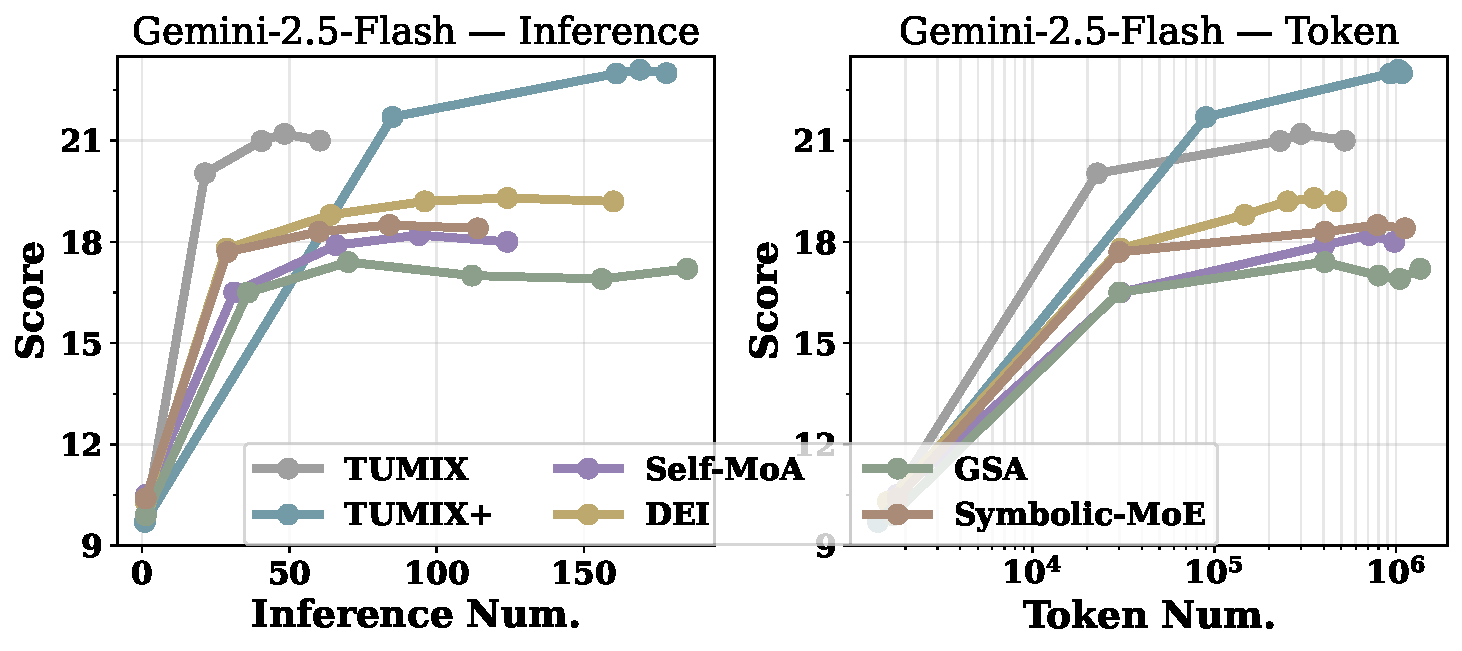
\includegraphics[width=0.8\linewidth]{Figures/scaling_flash_only.pdf}
   \caption{Scaling behavior of HLE scores in Gemini-2.5-flash relative to inference cost and total token count across different tool-augmented test-time scaling methods, where the token count includes both input and output tokens.}
   \label{fig:Scaling behavior of Gemini-2.5-flash}
\end{figure*}

\newpage
\section{LLM token confidence of generated responses}
\label{appendix sec: LLM token confidence of generated responses}
\begin{figure*}[ht]
  \centering
  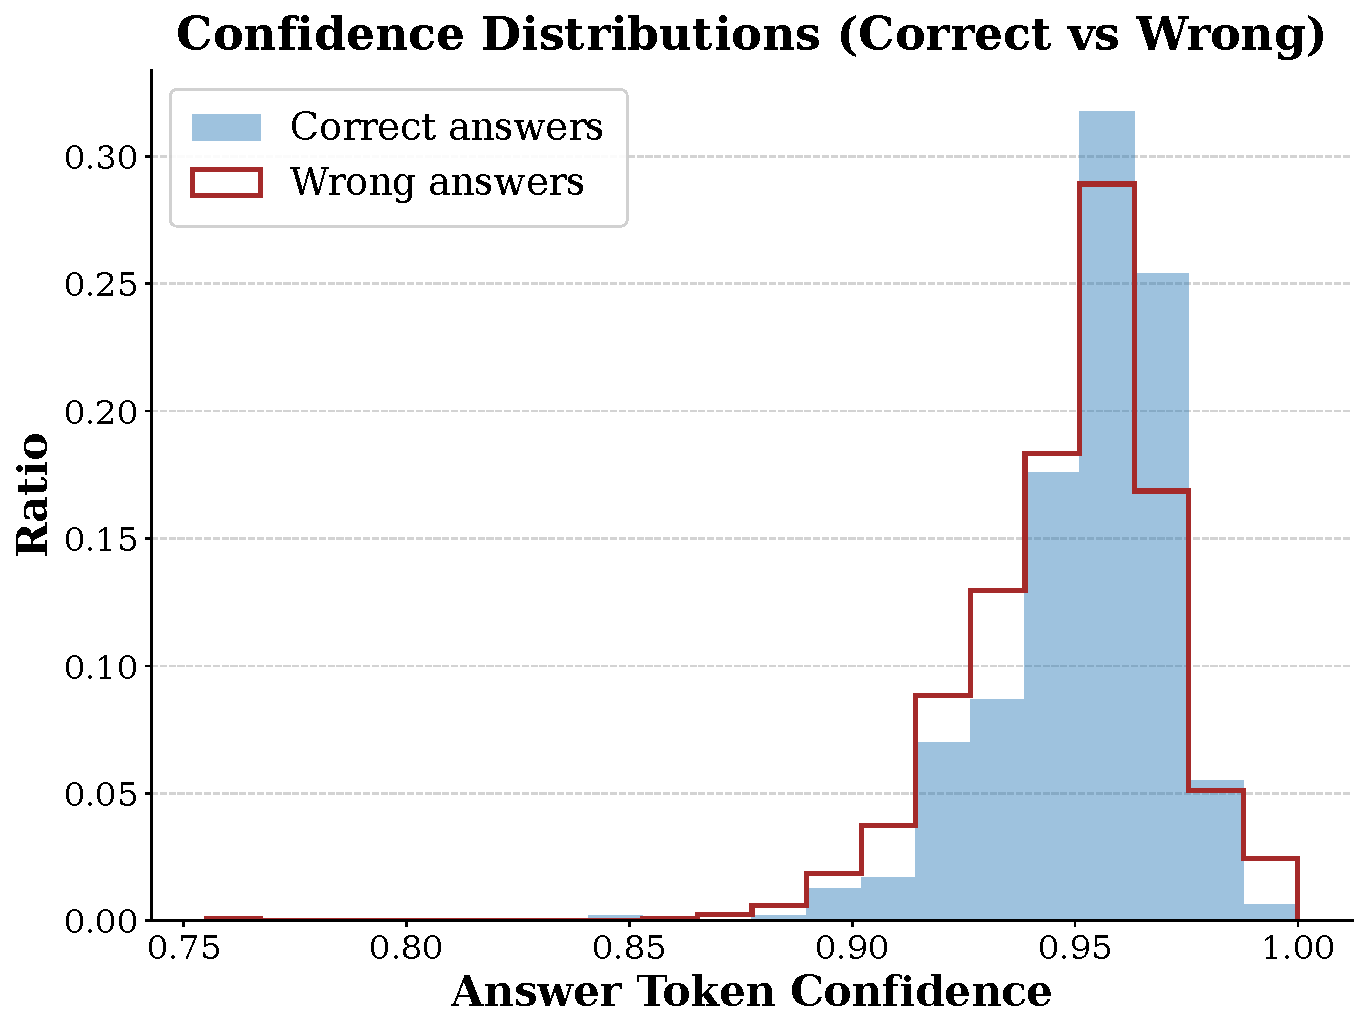
\includegraphics[width=0.7\linewidth]{Figures/logprob_compare.pdf}
   \caption{Distribution of LLM response confidence for correct and wrong answers. The response confidence is calculated based on the average token probability of the whole generated response. Here we use the responses of agent \texttt{CoT} as representative, as we find the distribution characteristics are very close among different agents.}
   \label{fig:logprob_compare}
\end{figure*}